
\section{Målgruppe}
Målgruppen for tjenesten er voksene privatpersoner som enten har bil eller eier en parkeringsplass. Dette vil si i aldersgruppen 18 til cirka 80 år. Næringsvirksomhet som har eiendom til disposisjon, skal også ha mulighet for å bruke tjenesten. Tjenesten skal være brukervennlig slik at alle i målgruppen kan på en enkel måte benytte seg av tilbudet. Vi har fokusert på privatpersoners bruk når vi har utviklet prototypen.

% Vår målgruppe er alle som har lappen eller bil og firmaer med parkeringsplasser ledig. Så aldermessig er det fra 18 år til 80 år. 
% Her skal det være brukervennlig og lett for de ulike personene å bruke det. 
% Vi har valgt to forskjellige brukergrupper å ta hensyn til. Vi har valgt å fokusere på privatpersoner og bedrifter som kan bruke tjenesten.


\subsection{Personas}
Personas er personer som blir funnet opp for å etterligne mulige brukere av tjenesten. Meningen med fiktive personer er å finne viktige funksjoner og krav i systemet utfra brukerens behov. Personas skal virke så ekte som mulig slik at de ligner på potensielle kunder. Hver personas bør være en unik person slik at det kan fås fram forskjellige krav utfra hver personas. Det er viktig å lage slike fiktive personer under utvikling av en tjeneste slik at man tidlig kan avdekke brukerens behov til tjenesten. Ved å lage personas er det mye lettere å se for seg hva som trengs i systemet ettersom at man kan se krav i systemet fra brukerens perspektiv.  



Vi har laget forskjellige personas til de forskjellige brukergruppene. Disse er igjen delt opp i alder for å avdekke forskjellige krav og brukermønster. 
%Ved å bruke personas kan vi se hvilke funksjoner og behov som trengs fra tjenesten og i hvilke situasjoner hver enkelte brukere vi benytte seg av den. 

% Vi har laget personas for de to forskjellige brukergrupper. Vi har deretter delt disse opp i alder for å avdekke forskjellige krav. 
% Ved å ha personas kan vi se på hva slags funksjoner som trengs og hvordan de samhandler med tjenesten.


\subsubsection{Privatperson}
For privatpersoner er det fire personas som er i forskjellige alder.


\vspace{1em}
\textbf{\underline{Siri Kristiansen}}
\vspace{-1em}
\begin{description}[style=multiline,leftmargin=2.2cm]
\item[Alder:] 23
\item[Arbeid:] Nyutdannet sykepleier på Rikshospitalet
\item[Sivilstatus:] Singel
\end{description}

\vspace{1em}
\noindent \textbf{\underline{Simon Berger}}
\vspace{-1em}
\begin{description}[style=multiline,leftmargin=2.2cm]
\item[Alder:] 34
\item[Arbeid:] Finansanalytiker hos BANE Nord
\item[Sivilstatus:] Gift med to barn
\end{description}



\vspace{1em}
\noindent \textbf{\underline{Jørn Jensen}}
\vspace{-1em}
\begin{description}[style=multiline,leftmargin=2.2cm]
\item[Alder:] 70
\item[Arbeid:] Pensjonert
\item[Sivilstatus:] Gift 
\end{description}


\vspace{1em}
\noindent \textbf{\underline{Bård Kronvol}}
\vspace{-1em}
\begin{description}[style=multiline,leftmargin=2.2cm]
\item[Alder:] 55
\item[Arbeid:] IKT for kommunen
\item[Sivilstatus:] Nyskilt med barn
\end{description}


\subsubsection{Bedrifter}
% For bedrifter har vi valgt en leder i en bedrift. Det er for å vise at firmaet styres av en person/direktør. Det viser også til at et firma har da en person som har ansvar for parkeringsplassen for tjenesten. 
% 

\vspace{1em} 
\noindent\textbf{\underline{Arne Arnolfsen}}
\vspace{-1em}
\begin{description}[style=multiline,leftmargin=2.2cm]
\item[Alder:] 45
\item[Arbeid:]  Eier av en lokal rørleggerbedrift.
\item[Sivilstatus:] Enkemann

\end{description}



\subsection{Brukerhistorie}
Brukerhistorier er korte historier som beskriver en person og et dilemma der de kan ha nytte av systemet. Ulike mennesker har forskjellige syn på bruk av systemet, og med brukerhistorier vil det gi en felles forståelse med tanke på videre utvikling av systemet.

\subsubsection{Privatpersoner}
\textit{Simon Berger}, er en travel person som jobber i finansmiljøet i Oslo. Han bor i utkanten av byen, på Jar i Bærum sammen med sin kone og to barn. Barna er i barnehagealder, og for at Simon skal rekke å hente barna etter jobb er han nødt til å bruke bil – kollektiv tar for lang tid. I nærheten av jobben er det ikke tilgjengelige plasser, og jobben tilbyr ikke de ansatte parkering. Det blir fort dyrt for Simon å parkere i parkeringshus hver dag. Så han skulle ønske det var en mulighet for å parkere rimeligere i byen mens han er på jobb.



\textit{Siri Kristiansen} er en nyutdannet sykepleier som jobber på Rikshospitalet. Hun er nettopp ferdig med studier, og bor fortsatt i byen sammen med venninnen Kari. Som nyutdannet er økonomien trang, men hun er heldig som har klart å kjøpe seg en leilighet. Hun leier ut ett rom til venninnen Kari for å få ting til å gå rundt. Hun kunne tenkte seg å tjene noen ekstra kroner, slik at hverdagen blir litt enklere. Verken Kari eller Siri disponerer bil, men leiligheten Siri eier disponerer en parkeringsplass, denne står for det meste tom, og brukes kun de få gangene de får gjester på besøk, som er på ettermiddagen eller i helgene.  


\textit{Jørn Jensen} er en pensjonert mann som liker å være sosial. Han og kona får tilbud om å gå på Dagsenter i Halden, som han elsker å gjøre. Der får han sitte lenge og skravle med andre eldre. Kona Kjersti har problemer med å gå, og de bor to timers gangavstand unna Dagsenteret slik at de bruker bil for å komme dit. Dagsenteret har få parkeringsplasser, og de er alltid opptatt. Jørn ønsker da en parkeringsplass de kan leie i et gitt tidsrom for en rimelig sum, slik at de kan komme seg til Dagsenteret.



\textit{Bård Krovold} er IKT-ansvarlig i kommunen han jobber for og stortrives med å ha noe og fikse på. Bård er nyskilt og barna hans har flyttet ut, dermed sitter Bård igjen alene i ett større hus sentralt i Oslo med to parkeringsplasser hvor han kun trenger en, og i ukedagene er ofte begge ledig. Ved å leie ut den ekstra parkeringsplassen vil Bård få noen ekstra kroner han kan bruke på hobbyene sine, og kanskje han kan bli kjent med noen nye samtidig. 

\subsubsection{Bedrift}

% \textit{Arne Arnolfsen} er en arbeider med godt mot. Han elsker jobben sin, og etter konas død er det hans eneste positive i hans liv. Etter at en bedrift kansellerte en bestilling av parkeringhus har Arne lurt på hva som skal skje med parkeringshuset som de bygde før kanselleringen. Huset er lite og de har vanskelig å selge det videre til andre bedrifter. Arne dermed ønsker å leie parkeringsplassene ut for en rimelig pris for å ikke tape penger på parkeringshuset som ble bygd.

\textit{Arne Arnolfsen} er en arbeider med godt mot. Han elsker jobben sin, og etter konas død er det hans eneste positive i hans liv. Rørleggerbedriften har holdt til i samme lokaler sentralt i Oslo i mange år. Og er heldige som har en stor parkeringsplass hvor alle firmabilene står parkert over natten. På dagtid står de fleste av disse plassene tomme, for arbeiderne er ute på jobb hos kunder med bilene. Arne er en kremmer, så han lurer på om det er mulig å leie ut disse plassene på dagtid.


\subsection{User Case}
\label{user_case}
User Case er en beskrivelse på hvordan en person skal bruke en del av systemet. I hvert user case blir en av personas brukt til å beskrive en situasjon basert på funksjoner i systemet. Beskrivelsen til en user case bør være så spesifikk som mulig for å kunne få fram interaksjoner mellom brukeren og systemet. Dette hjelper med å finne hvordan forskjellige funksjoner skal implementeres og hvordan deler av systemet skal fungere utfra brukerens opplevelse.  
%Fordypning av usercase og hva man får ut av det.


I tabellene \ref{tab:leie_Jørn}, \ref{tab:Siri_leggeut},  \ref{tab:simon_søk_parkeringsplass}, \ref{tab:bård_se_oversikt} og \ref{tab:arne_leggeparkering} ser man user casene til de ulike funksjonene som våres personas ønsker å se og bruke.


\begin{table}[H]
\begin{tabularx}{\textwidth}{r|X}
\textbf{System}      & Utleie av parkeringsplasser. \\ [.5em]
\textbf{Use case}    & Leie parkeringsplass. \\ [.5em]
\textbf{Aktor}       & Jørn Jensen  \\ [.5em]
\textbf{Krav}        & Bruker må være på nettsiden og logget inn. \\ [.5em]
\textbf{Trigger}     & Å kunne finne ledig parkeringsplass. \\ [.5em]
\textbf{Beskrivelse} & Brukeren åpner nettsiden og logger inn. Deretter trykker brukeren på «se tilgjengelig parkeringsplasser» for å  komme til siden for tilgjengelige parkeringsplasser. Der fyller han inn informasjonen om hvor parkeringsplassen skal befinne seg, og får med det opp alle ledige plasser i området. Brukeren velger så den plassen han vil ha og går videre til betalingssiden. Der får han opp plassen han ønsker å leie og prisen. Så velger han foretrukket betalingsmåte, Vipps eller Mastercard. Deretter blir han ført til tredjepartens betalingsside og betaler der. Når brukeren har betalt og betalingen er godkjent så blir han ført tilbake til betalingssiden. Her får brukeren en bekreftelse på siden om at parkeringsplassen er betalt for og nå er aktiv. \vspace{0.5em} \\ 
\textbf{Stimuli}     & Leid parkeringsplass. \\ [.5em]
\textbf{Respons}     & Mottar bekreftelse om at betaling er godkjent, deretter blir  parkeringsplassen utlånt til brukeren og utilgjengelig for andre brukere.        
\end{tabularx}
    \caption{User Case for å leie parkeringsplass }
    \label{tab:leie_Jørn}
\end{table}


\begin{table}[H]
\begin{tabularx}{\textwidth}{r|X}
\textbf{System}      & Utleie av parkeringsplasser. \\ [.5em]
\textbf{Use case}    & Legge ut parkeringsplass.  \\ [.5em]
\textbf{Aktor}       & Siri Kristiansen  \\ [.5em]
\textbf{Krav}        & Bruker må være innlogget inn i tjenesten. \\ [.5em]
\textbf{Trigger}     & Lyst til å legge ut en parkeringsplass til leie. \\ [.5em]
\textbf{Beskrivelse} & Brukeren åpner nettsiden og logger inn. Deretter  trykker brukeren på «lei ut parkeringsplass» for å komme til siden for å legge til sin parkeringsplass. Der fyller hun ut all informasjonen om parkeringsplassen som pris, lokasjon og tilgjengelighet. Så legger hun den til og får en bekreftelse om at parkeringsplassen er opprettet og gjort tilgjengelig på siden. \vspace{0.5em} \\ 
\textbf{Stimuli}     & Legger ut parkeringsplass i tjenesten. \\ [.5em]
\textbf{Respons}     & Parkeringsplassen har blitt lagt ut og vises i lei parkeringsplass.         
\end{tabularx}
    \caption{User Case for å lage parkeringsplass}
    \label{tab:Siri_leggeut}
\end{table}



\begin{table}[H]
\begin{tabularx}{\textwidth}{r|X}
\textbf{System}      & Utleie av parkeringsplasser. \\ [.5em]
\textbf{Use case}    & Søke opp parkeringsplasser.  \\ [.5em]
\textbf{Aktor}       & Simon Berger  \\ [.5em]
\textbf{Krav}        & Bruker må være innlogget inn i tjenesten. \\ [.5em]
\textbf{Trigger}     & Ønsker å finne parkeringsplasser i Oslo.\\ [.5em]
\textbf{Beskrivelse} & Brukeren åpner nettsiden og logger inn. Deretter trykker brukeren på «se tilgjengelig parkeringsplasser» for å  komme til siden for tilgjengelige parkeringsplasser. Der fyller brukeren inn informasjonen om hvor  parkeringsplassen skal befinne seg, og får med det opp alle ledige plasser i området. Finner brukeren en ledig plass legger han den til og føres videre  til betalingssiden. Der får han opp plassen han ønsker å leie og prisen. Så velger han foretrukket betalingsmåte, Vipps eller Mastercard. Deretter blir han ført til tredjepartens betalingsside og betaler der. Når brukeren har betalt og betalingen er godkjent så blir han ført tilbake til betalingssiden. Her får brukeren en bekreftelse på siden om at parkeringsplassen er betalt for og nå er aktiv. \vspace{0.5em} \\ 
\textbf{Stimuli}     & Finner parkeringsplass i området. \\ [.5em]
\textbf{Respons}     & Mottar bekreftelse om at betaling er godkjent, deretter blir  parkeringsplassen utlånt til brukeren og utilgjengelig for andre brukere.
\end{tabularx}
    \caption{User Case for å søke opp parkeringsplass}
    \label{tab:simon_søk_parkeringsplass}
\end{table}

\begin{table}[H]
\begin{tabularx}{\textwidth}{r|X}
\textbf{System}      & Utleie av parkeringsplasser. \\ [.5em]
\textbf{Use case}    & Se oversikt over inntekter.  \\ [.5em]
\textbf{Aktor}       & Bård Kronvold   \\ [.5em]
\textbf{Krav}        & Bruker må være innlogget inn i tjenesten \\ [.5em]
\textbf{Trigger}     & Ønsker å se inntektene over sin parkeringsplass \\ [.5em]
\textbf{Beskrivelse} & Brukeren åpner nettsiden og logger inn. Deretter trykker brukeren på  "min side", og kommer til siden hvor han kan se oversikten over inntektene sine for parkeringsplassene. Brukeren kan da velge å se oversikten over alle parkeringsplassene, eller en bestemt parkeringsplass. \vspace{0.5em} \\ 
\textbf{Stimuli}     & Finne hvor mye inntekter brukeren får.\\ [.5em]
\textbf{Respons}     & Ser da hvor mye inntekter han får på den ene  parkeringsplassen som han har.
\end{tabularx}
    \caption{User Case for å se oversikt}
    \label{tab:bård_se_oversikt}
\end{table}


\begin{table}[H]
\begin{tabularx}{\textwidth}{r|X}
\textbf{System}      & Utleie av parkeringsplasser. \\ [.5em]
\textbf{Use case}    &  Legge ut flere parkeringsplasser på siden.  \\ [.5em]
\textbf{Aktor}       & Arne Arnolfsen    \\ [.5em]
\textbf{Krav}        & Være innlogget på sin profil og være registrert som firma. Parkeringsplassene må være mulig å legge til. Må ha betalt den månedlige prisen \vspace{0.5em} \\ 
\textbf{Trigger}     &  Ønske å legge ut parkeringsplassene  \\ [.5em]
\textbf{Beskrivelse} & Brukeren åpner nettsiden og logger inn. Deretter trykker brukeren på «lei ut parkeringsplass» for å komme til siden for å legge til sin parkeringsplass. Der fyller brukeren ut all informasjonen om parkeringsplassen og legger den til. Her får firmabrukeren en bekreftelse på siden om at parkeringsplassen er betalt for og nå er tilgjengelig for andre å leie.  \vspace{0.5em} \\ 
\textbf{Stimuli}     & Legger ut parkeringsplassen offentlig så andre kan leie den. \vspace{0.5em}\\ 
\textbf{Respons}     & Bekrefter at parkeringsplassen har blitt lagt ut og gjort tilgjengelig i systemet.
\end{tabularx}
    \caption{User Case for å legge ut parkeringsplasser for firmaet}
    \label{tab:arne_leggeparkering}
\end{table}





\newpage
\subsection{User Case Diagram}

\begin{figure}[H]
    \centering
    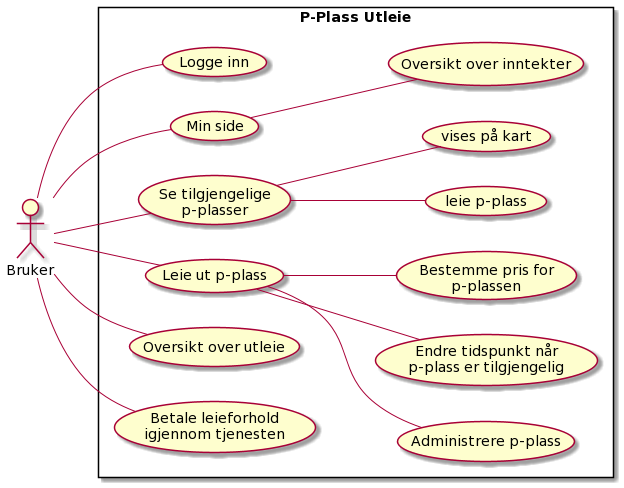
\includegraphics[width=\textwidth]{bilder/uml/usercase_diagram.png}
    \caption{User case diagram med forskjellige funksjoner for tjenesten}
    \label{fig:user_case}
\end{figure}
% Omskrive ! 
Ut ifra disse User Case, personas og brukerhistorie kom vi fram til dette user case diagrammet med forskjellige ønsket funksjonaliteter. 
Det ser du i Figur \ref{fig:user_case}.
Fra denne figuren kan man finne ulike krav som vi setter til systemet.
